

\begin{document}

This section covers the design choices associated with the various circuits constructed. The individual circuits designed were a Schmitt trigger configured op amp as the signal conditioner and an op amp driving a BJT for the current driver. The input waveform was generated using the ring oscillator from Lab 3. A voltage regulator supplied a steady 5V from a 9V battery source.

The order in which the circuits are discussed is as follows: first, the ring oscillator, followed by the signal conditioner, then the current driver, and then finally the voltage regulator.

\subsection{Ring oscillator}
\subfile{CircuitDevelopment/ring_oscillator.tex}

\subsection{Signal conditioner}
\subfile{CircuitDevelopment/signal_conditioner.tex}

\subsection{Current driver}
\subfile{CircuitDevelopment/current_driver.tex}

\subsection{Voltage regulator}
\subfile{CircuitDevelopment/voltageregulator.tex}


\subsection{Simulated summary}
The final simulated circuit is shown in Figure \ref{fig:finalschemlab4}.

\begin{figure}[H]
	\centering
	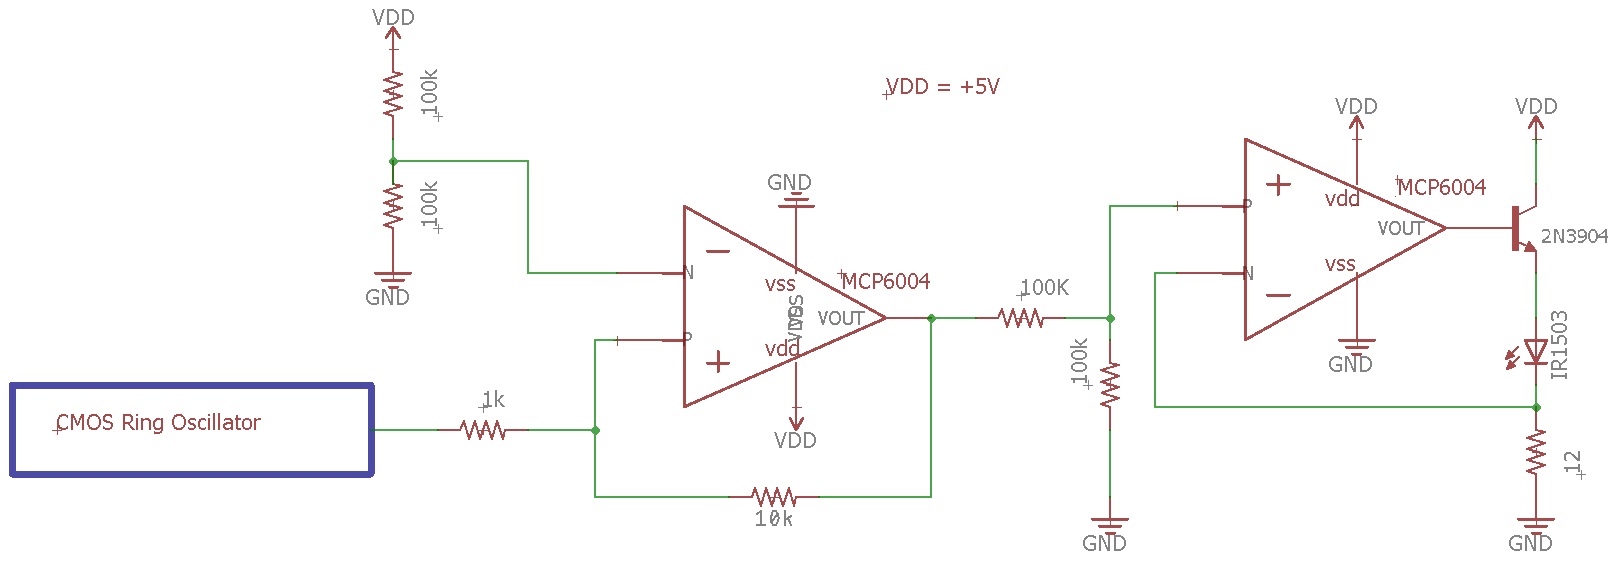
\includegraphics[width=0.7\linewidth]{CircuitDevelopment/FinalschemLab4}
	\caption[Simulated circuit]{Simulated LED driver}
	\label{fig:finalschemlab4}
\end{figure}
The summary of simulated results from this circuit is shown in Table \ref{tab:simresults}.

\begin{table}[H]
	\centering
\caption{Simulated Results}
\label{tab:simresults}
\begin{tabular}{|c|c|}
	\hline 
	Component & Simulated Values \\ 
	\hline 
	Conditioned Voltage & 5V \\ 
	\hline 
	Conditioned Frequency & 20kHz \\ 
	\hline 
	Conditioned Duty-Cycle & 48\% \\ 
	\hline 
	Output Current & 200mA \\ 
	\hline 
	R$_{sense}$ & 12$\Omega$ \\ 
	\hline 
\end{tabular} 
\end{table}

The simulated circuit operated as expected and provided enough current in order to drive the LED. The resulting waveform through the LED is the correct frequency and duty-cycle in order to detected by the optical uplink receiver.
	






\end{document}